\pagestyle{fancy}
\fancypagestyle{plain}{}
\cfoot{\Roman{chapter}-\arabic{page}}
\rhead{}
\setcounter{page}{1}
\chapter{METODOLOGI PENELITIAN}

\section{Pendahuluan}
Pada bab ini akan menjabarkan metodologi penelitian serta manajemen proyek penelitian yang akan
diimplementasikan pada penelitian ini. Tahapan penelitian akan dijadikan sebagai landasan untuk
setiap fase pengembangan perangkat lunak dan memberikan sebuah solusi berdasarkan rumusan masalah
untuk mencapai tujuan penelitian.

\section{Pengumpulan Data}~\label{sec:pengumpulan_data}
Dalam bagian ini akan diuraikan bagaimana tahapan penulis dalam melakukan pengumpulan data yang akan
digunakan dalam penelitian.

\subsection{Jenis Data}
Data yang digunakan dalam penelitian ini adalah jenis data primer. Data primer adalah data yang
diambil dari sumbernya langsung melalui sumber aslinya tanpa perantara. Jumlah data primer direncanakan
sebanyak 6.000 \emph{review}, dengan 3.000 berlabel positif dan 3.000 \emph{review} berlabel
negatif. Data tersebut akan digunakan untuk melatih CNN dalam melakukan analisis sentimen.

\subsection{Sumber Data}
Data primer yang akan digunakan untuk melaksanakan penelitian ini diperoleh dari \emph{review}
aplikasi gojek, grab, dan maxim yang ada di \emph{Google Play Store}. Data \emph{review} telah
dilabeli menjadi dua kelas, yaitu positif dan negatif secara otomatis berdasarkan skor dari
\emph{review} yang ada di \emph{Google Play Store} dengan ketentuan 1 adalah label negatif dan 5
adalah label positif~\citep{Akbar2022},~\citep{Smetanin2019},~\citep{Amanatidis2019}.\newpage


\pagestyle{fancy}
\fancypagestyle{plain}{}
\rhead{\Roman{chapter}-\arabic{page}}
\cfoot{}

\subsection{Metode Pengumpulan Data}
Pengumpulan data primer dilakukan dengan cara mengunduh yaitu \emph{crawling} di website
\emph{Google Play Store} dengan bantuan pustaka (\emph{library}) \emph{google-play-scraper}. Data
dikumpulkan dari \emph{review} 3 aplikasi angkutan online yaitu gojek, grab, dan maxim dengan kriteria
jumlah kata dalam kalimat minimal 11 kata. Masing-masing review dari 3 aplikasi tersebut diambil
1000 dengan skor 1 dan 1000 dengan skor 5.

\subsection{Contoh Data Sentimen}
Dalam bagian ini akan ditampilkan contoh data sentimen yang akan digunakan dalam penelitian ini
dalam bentuk tabel dapat dilihat pada Tabel~\ref{tab:contoh_data_sentimen}.

\begin{table}[H]
  \centering
  \caption{Contoh Data Sentimen}
  \label{tab:contoh_data_sentimen}
  \begin{tabularx}{\columnwidth}{|X|X|l|}
    \hline
    reviewId                             & content                                                                                                                                                                          & label   \\ \hline
    d4e7736d-f5ea-4c8e-af74-198266968a76 & Gk jelas aplikasi ini gk kaya punya sebelah lokasi tujuan udh di tulis yg keluar alamat lain.masa order blm ada tujuanya udh masuk kn bikin stres ampe emosi gw. Hancur pokoknya & Negatif \\ \hline
    a5a355f8-a208-44d6-8a7f-f255139d20fa & Gda LG kecuali gojek...top pokok y                                                                                                                                               & Positif \\ \hline
    3ad826e8-7f10-4854-9d16-3dd90eefbada & cpt banget                                                                                                                                                                       & Positif \\ \hline
    c7ded523-ead6-4bc3-aa2f-69b226e52d02 & Mending gojek aja                                                                                                                                                                & Negatif \\ \hline
  \end{tabularx}
\end{table}

Dan untuk jumlah sentimen yang bernilai positif dan negatif dapat dilihat pada Gambar~\ref{fig:bar_pos_neg}.
\begin{figure}[H]
  \centering
  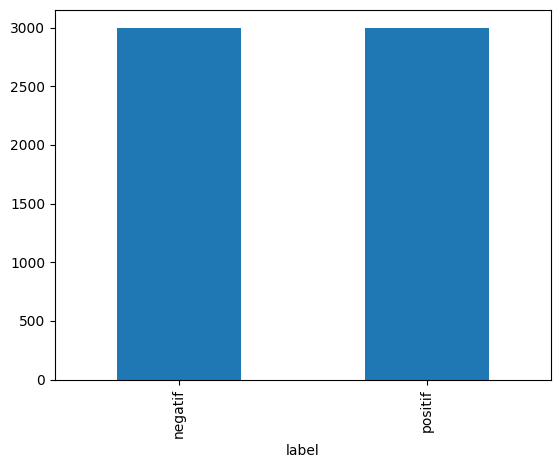
\includegraphics[scale=0.5]{assets/bar_pos_neg.png}
  \caption{Jumlah Sentimen Positif dan Negatif}
  \label{fig:bar_pos_neg}
\end{figure}

\section{Tahapan Penelitian}
Untuk mengetahui kinerja dari \emph{Convolutional Neural Network} pada klasifikasi sentimen, maka
penelitian ini dilakukan dengan tahapan pada penelitian seperti pada Gambar~\ref{fig:diagram_tahapan_penelitian}.

\begin{figure}[H]
  \centering
  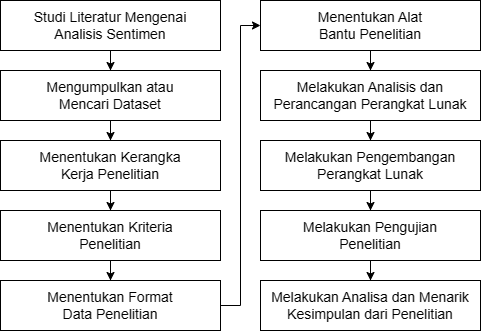
\includegraphics[scale=0.59]{assets/diagram_tahapan_penelitian.png}
  \caption{Diagram Tahapan Penelitian}
  \label{fig:diagram_tahapan_penelitian}
\end{figure}

\subsection{Studi Literatur Mengenai Analisis Sentimen}
Dalam tahapan penelitian ini penulis melakukan studi literatur mengenai analisis sentimen. Penulis
menganalisa, memahami, mengumpulkan semua sumber yang berkaitan dengan analisis sentimen dengan
tujuan untuk mendapatkan landasan dalam penelitian yang dilakukan. Dengan didapatkannya landasan yang
memiliki relevansi pada permasalahan yang diteliti diharapkan nantinya dapat membantu dalam proses
penelitian.

\subsection{Mengumpulkan / Mencari Dataset}
Dalam tahapan penelitian ini penulis melakukan pengumpulan data dengan dua tujuan yang pertama adalah
untuk melatih model CNN dalam analisis sentimen, dan yang terakhir adalah untuk mempermudah penanganan
bahasa gaul. CNN dengan model yang baik dapat diperoleh dengan cara melatih CNN menggunakan banyak
data. Semakin banyak data yang dapat digunakan untuk melatih CNN maka model dari CNN akan menjadi
lebih akurat.

\subsection{Kerangka Kerja Penelitian}
Analisis sentimen dalam penelitian ini akan dijalankan beberapa tahapan, yaitu studi literatur
untuk memahami permasalahan yang diteliti, persiapan data agar dapat diimplementasikan kedalam program,
pra-pengolahan data, proses latih data menggunakan metode CNN, analisis hasil, dan penarikan kesimpulan.
Kerangka kerja penelitian dapat dilihat pada Gambar~\ref{fig:kerangka_kerja_penelitian}.

\begin{figure}[H]
  \centering
  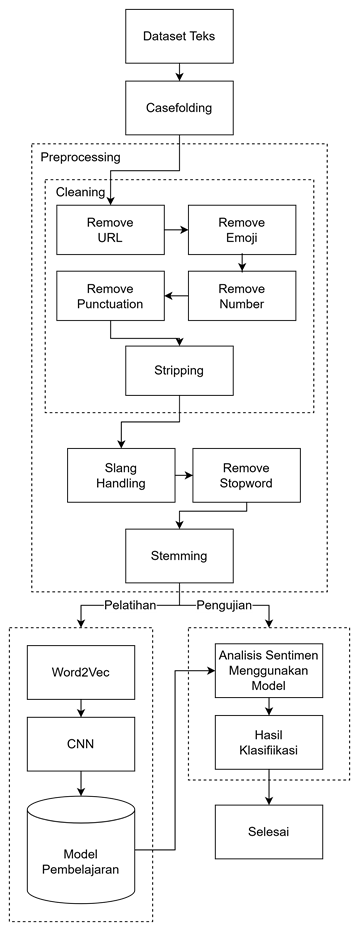
\includegraphics[width=\textwidth, height=15cm, keepaspectratio]{assets/kerangka_kerja_penelitian.png}
  \caption{Kerangka Kerja Penelitian}
  \label{fig:kerangka_kerja_penelitian}
\end{figure}

Berdasarkan kerangka kerja pada Gambar~\ref{fig:kerangka_kerja_penelitian}, analisis sentimen menggunakan
CNN memiliki tahapan sebagai berikut.

\begin{enumerate}
  {\bfseries \item Praproses Teks}\\
  Langkah pertama yang dilakukan dalam penelitian ini adalah praproses teks. Pada tahapan ini teks
  diubah ke huruf kecil (\emph{casefolding}), teks akan dihilangkan \emph{URL} (\emph{URL Removal}),
  dihilangkan emotikon, dihilangkan angka, dihilangkan tanda baca. Dilanjutkan dengan penanganan
  bahasa gaul, dihilangkan \emph{stopword}, diubah menjadi kata dasar atau \emph{stemming}, dan \emph{tokenizing}.
  Untuk penjelasan yang lebih detail pada langkah-langkah praproses dapat dilihat pada~\autoref{Praproses}.

  \begin{enumerate}
    {\bfseries \item \emph{Casefolding}}\\
    Langkah pertama dalam praproses adalah casefolding, casefolding merupakan teknik merubah semua
    huruf didalam teks menjadi seragam umumnya adalah huruf kecil. Contoh kalimat sebelum dilakukan
    \emph{casefolding} dan yang sudah dilakukan \emph{casefolding} dapat dilihat pada Tabel~\ref{tab:contoh_casefolding}

    \begin{table}[H]
      \centering
      \caption{Contoh \emph{Casefolding}}
      \label{tab:contoh_casefolding}
      \begin{tabularx}{\columnwidth}{|X|X|}
        \hline
        content                                                                                                                                                                                      & lowercased                                                                                                                                                                                   \\ \hline
        {\bfseries Gk} jelas aplikasi ini gk kaya punya sebelah lokasi tujuan udh di tulis yg keluar alamat lain.masa order blm ada tujuanya udh masuk kn bikin stres ampe emosi gw. Hancur pokoknya & {\bfseries gk} jelas aplikasi ini gk kaya punya sebelah lokasi tujuan udh di tulis yg keluar alamat lain.masa order blm ada tujuanya udh masuk kn bikin stres ampe emosi gw. hancur pokoknya \\ \hline
        {\bfseries Gda LG} kecuali gojek...top pokok y                                                                                                                                               & {\bfseries gda lg} kecuali gojek...top pokok y                                                                                                                                               \\ \hline
        cpt banget                                                                                                                                                                                   & cpt banget                                                                                                                                                                                   \\ \hline
        {\bfseries Mending} gojek aja                                                                                                                                                                & {\bfseries mending} gojek aja                                                                                                                                                                \\ \hline
      \end{tabularx}
    \end{table}

    {\bfseries \item \emph{Cleaning}}\\
    Langkah selanjutnya adalah pembersihan teks dari karakter yang tidak diperlukan. Langkah-langkah
    dalam tahapan \emph{cleaning} ini yaitu, \emph{Remove URL}, \emph{Remove Emoji}, \emph{Remove Number},
    \emph{Remove Punctuation}, dan \emph{Stripping} untuk penjelasan lebih detil pada tahapan cleaning
    dapat dilihat pada~\autoref{Praproses}. Contoh kalimat sebelum dilakukan \emph{cleaning} dan yang
    sudah dilakukan \emph{cleaning} dapat dilihat pada Tabel~\ref{tab:contoh_cleaning}.

    \begin{table}[H]
      \centering
      \caption{Contoh \emph{Cleaning}}
      \label{tab:contoh_cleaning}
      \begin{tabularx}{\columnwidth}{|X|X|}
        \hline
        lowercased                                                                                                                                                                       & cleaned                                                                                                                                                                          \\ \hline
        gk jelas aplikasi ini gk kaya punya sebelah lokasi tujuan udh di tulis yg keluar alamat lain.masa order blm ada tujuanya udh masuk kn bikin stres ampe emosi gw. hancur pokoknya & gk jelas aplikasi ini gk kaya punya sebelah lokasi tujuan udh di tulis yg keluar alamat lain masa order blm ada tujuanya udh masuk kn bikin stres ampe emosi gw  hancur pokoknya \\ \hline
        gda lg kecuali gojek \underline{\ldots} top pokok y                                                                                                                              & gda lg kecuali gojek top pokok y                                                                                                                                                 \\ \hline
        cpt banget                                                                                                                                                                       & cpt banget                                                                                                                                                                       \\ \hline
        mending gojek aja                                                                                                                                                                & mending gojek aja                                                                                                                                                                \\ \hline
      \end{tabularx}
    \end{table}

    {\bfseries \item \emph{Slang Handling}}\\
    Langkah selanjutnya adalah mengubah kata gaul menjadi kata formalnya dengan menggunakan kamus alay
    hasil dari penelitian \citet{Aliyah2018}. Contoh kalimat sebelum dilakukan \emph{slang handling}
    dan yang sudah dilakukan \emph{slang handling} dapat dilihat pada Tabel~\ref{tab:contoh_slang_handling}.

    \begin{table}[H]
      \centering
      \caption{Contoh \emph{Slang Handling}}
      \label{tab:contoh_slang_handling}
      \begin{tabularx}{\columnwidth}{|X|X|}
        \hline
        cleaned                                                                                                                                                                                                                                                                          & slang\_handled                                                                                                                                                                                                                                                                                       \\ \hline
        {\bfseries gk} jelas aplikasi ini {\bfseries gk kaya} punya sebelah lokasi tujuan {\bfseries udh} di tulis yg keluar alamat lain masa order {\bfseries blm} ada tujuanya {\bfseries udh} masuk {\bfseries kn} bikin stres {\bfseries ampe} emosi {\bfseries gw}  hancur pokoknya & {\bfseries enggak} jelas aplikasi ini {\bfseries enggak kayak} punya sebelah lokasi tujuan {\bfseries sudah} di tulis yang keluar alamat lain masa order {\bfseries belum} ada tujuanya {\bfseries sudah} masuk {\bfseries kan} bikin stres {\bfseries sampai} emosi {\bfseries gue} hancur pokoknya \\ \hline
        {\bfseries gda lg} kecuali gojek top pokok {\bfseries y}                                                                                                                                                                                                                         & {\bfseries enggak ada lagi} kecuali gojek top pokok {\bfseries ya}                                                                                                                                                                                                                                   \\ \hline
        {\bfseries cpt} banget                                                                                                                                                                                                                                                           & {\bfseries cepat} banget                                                                                                                                                                                                                                                                             \\ \hline
        mending gojek {\bfseries aja}                                                                                                                                                                                                                                                    & mending gojek {\bfseries saja}                                                                                                                                                                                                                                                                       \\ \hline
      \end{tabularx}
    \end{table}

    {\bfseries \item \emph{Stopword Removal}}\\
    Langkah selanjutnya adalah menghilangkan kata yang tidak memiliki makna dari kalimat, proses ini
    dilakukan dengan bantuan pustaka (\emph{library}) Sastrawi. Contoh kalimat sebelum dilakukan
    \emph{stopword removal} dan yang sudah dilakukan \emph{stopword removal} dapat dilihat
    pada Tabel~\ref{tab:contoh_stopword_removal}.

    \begin{table}[H]
      \centering
      \caption{Contoh \emph{Stopword Removal}}
      \label{tab:contoh_stopword_removal}
      \begin{tabularx}{\columnwidth}{|X|X|}
        \hline
        slang\_handled                                                                                                                                                                                                                                                                                                   & stopword\_removed                                                                                      \\ \hline
        {\bfseries enggak jelas} aplikasi {\bfseries ini enggak} kayak {\bfseries punya} sebelah lokasi tujuan {\bfseries sudah di} tulis {\bfseries yang keluar} alamat {\bfseries lain masa} order {\bfseries belum ada} tujuanya {\bfseries sudah masuk kan} bikin stres {\bfseries sampai} emosi gue hancur pokoknya & aplikasi kayak sebelah lokasi tujuan tulis alamat order tujuanya bikin stres emosi gue hancur pokoknya \\ \hline
        {\bfseries enggak ada lagi} kecuali gojek top pokok {\bfseries ya}                                                                                                                                                                                                                                               & kecuali gojek top pokok                                                                                \\ \hline
        cepat banget                                                                                                                                                                                                                                                                                                     & cepat banget                                                                                           \\ \hline
        mending gojek {\bfseries saja}                                                                                                                                                                                                                                                                                   & mending gojek                                                                                          \\ \hline
      \end{tabularx}
    \end{table}

    {\bfseries \item \emph{Stemming}}\\
    Langkah selanjutnya adalah mengubah kata yang ada didalam kalimat menjadi kata dasarnya, proses ini
    dilakukan dengan bantuan pustaka (\emph{library}) Sastrawi. Contoh
    kalimat sebelum dilakukan \emph{stemming} dan yang sudah dilakukan \emph{stemming} dapat dilihat
    pada Tabel~\ref{tab:contoh_stemming}.

    \begin{table}[H]
      \centering
      \caption{Contoh \emph{Stemming}}
      \label{tab:contoh_stemming}
      \begin{tabularx}{\columnwidth}{|X|X|}
        \hline
        stopword\_removed                                                                                                              & stemmed                                                                                                                 \\ \hline
        aplikasi kayak {\bfseries sebelah} lokasi {\bfseries tujuan} tulis alamat order tujuanya bikin stres emosi gue hancur pokoknya & aplikasi kayak {\bfseries belah} lokasi {\bfseries tuju} tulis alamat order tujuanya bikin stres emosi gue hancur pokok \\ \hline
        kecuali gojek top pokok                                                                                                        & kecuali gojek top pokok                                                                                                 \\ \hline
        cepat banget                                                                                                                   & cepat banget                                                                                                            \\ \hline
        mending gojek                                                                                                                  & mending gojek                                                                                                           \\ \hline
      \end{tabularx}
    \end{table}

    {\bfseries \item \emph{Tokenizing}}\\
    Langkah selanjutnya adalah memecah kalimat menjadi kumpulan kata, kata dipecah pada setiap spasi.
    Contoh kalimat sebelum dilakukan \emph{Tokenizing} dan yang sudah
    dilakukan \emph{Tokenizing} dapat dilihat pada Tabel~\ref{tab:contoh_tokenizing}.

    \begin{table}[H]
      \centering
      \caption{Contoh \emph{Tokenizing}}
      \label{tab:contoh_tokenizing}
      \begin{tabularx}{\columnwidth}{|X|X|}
        \hline
        stemmed                                                                                         & tokenized                                                                                                       \\ \hline
        aplikasi kayak belah lokasi tuju tulis alamat order tujuanya bikin stres emosi gue hancur pokok & [aplikasi, kayak, belah, lokasi, tuju, tulis, alamat, order, tujuanya, bikin, stres, emosi, gue, hancur, pokok] \\ \hline
        kecuali gojek top pokok                                                                         & [kecuali, gojek, top, pokok]                                                                                    \\ \hline
        cepat banget                                                                                    & [cepat, banget]                                                                                                 \\ \hline
        mending gojek                                                                                   & [mending, gojek]                                                                                                \\ \hline
      \end{tabularx}
    \end{table}
  \end{enumerate}

  {\bfseries \item Membagi Data Latih dan Data Uji}\\
  Setelah kata dijadikan token dataset akan dibagi umumnya dataset dibagi menjadi 3, data latih,
  data validasi dan data uji. Dataset berjumlah 6000 dibagi menjadi 60:20:20 ke data latih, data validasi,
  dan data uji sehingga jumlah data latih menjadi 4800 data, dan data uji menjadi 1200 data.

  {\bfseries \item \emph{Word2Vec}}\\
  \emph{Word2Vec} adalah salah satu cara untuk melakukan \emph{word embedding} yang berguna untuk
  merepresentasikan kata menjadi vektor bernilai rill~\citep{Khattak2019}. \emph{Word2Vec} yang
  digunakan pada penelitian ini adalah \emph{pre-trained Word2Vec} yang didapatkan dari \emph{website kaggle}
  \url{https://www.kaggle.com/datasets/bhimantoros/pretrained-word2vec-indonesia}.
  \emph{Word2Vec} tersebut dilatih dengan menggunakan \emph{dump} dari Wikipedia Bahasa Indonesia (\emph{latest})
  dengan parameter $vector\_size=400$ dan $window=5$.

  {\bfseries \item \emph{Word Embedding}}\\
  Tahapan selanjutnya adalah mengubah token menjadi bentuk \emph{word embedding} menggunakan
  model \emph{Word2Vec}. Jika didalam \emph{Word2Vec} terdapat kata tersebut maka nilai vektor
  \emph{word embedding} didalam \emph{Word2Vec} yang digunakan untuk menjadi bobot kata tersebut. Namun
  jika kata tersebut tidak terdapat didalam \emph{Word2Vec} maka nilai tersebut akan digantikan dengan
  nilai vektor nol dengan panjang yang sama. Kata yang telah diubah menjadi vektor tersebut dapat
  dicari kata yang memiliki makna yang serupa atau mirip dengan menggunakan persamaan \emph{cosine similarity} contoh
  hasil kata yang dilakukan \emph{cosine similarity} dapat dilihat pada Tabel~\ref{tab:contoh_word_embedding}.

  \begin{longtable}[c]{|l|l|l|}
    \caption{Contoh Word Embedding}
    \label{tab:contoh_word_embedding}                                     \\
    \hline
    Kata                          & Kata yang Mirip & Nilai Kemiripan     \\ \hline
    %
    \endhead
    \hline
    \endfoot
    %
    \multirow[t]{10}{*}{aplikasi} & browser         & 0.7291104793548584  \\ \cline{2-3}
                                  & plugin          & 0.706239640712738   \\ \cline{2-3}
                                  & Aplikasi        & 0.7045372724533081  \\ \cline{2-3}
                                  & software        & 0.6958788633346558  \\ \cline{2-3}
                                  & server          & 0.685064435005188   \\ \cline{2-3}
                                  & peramban        & 0.6805809736251831  \\ \cline{2-3}
                                  & perangkat       & 0.6803056001663208  \\ \cline{2-3}
                                  & desktop         & 0.6744617819786072  \\ \cline{2-3}
                                  & pengguna        & 0.6634056568145752  \\ \cline{2-3}
                                  & antarmuka       & 0.660811185836792   \\ \hline
    \multirow[t]{10}{*}{kayak}    & kano            & 0.7113837003707886  \\ \cline{2-3}
                                  & selancar        & 0.639840304851532   \\ \cline{2-3}
                                  & mendayung       & 0.6360390186309814  \\ \cline{2-3}
                                  & snorkeling      & 0.6303792595863342  \\ \cline{2-3}
                                  & sampan          & 0.6169499158859253  \\ \cline{2-3}
                                  & mancing         & 0.5901890993118286  \\ \cline{2-3}
                                  & diving          & 0.5830395221710205  \\ \cline{2-3}
                                  & berperahu       & 0.5679073929786682  \\ \cline{2-3}
                                  & camping         & 0.5665735006332397  \\ \cline{2-3}
                                  & mengayuh        & 0.5514955520629883  \\ \hline
    \multirow[t]{10}{*}{belah}    & kubu            & 0.4585886299610138  \\ \cline{2-3}
                                  & saling          & 0.4301983714103699  \\ \cline{2-3}
                                  & ujungnya        & 0.42498528957366943 \\ \cline{2-3}
                                  & sisinya         & 0.4137492775917053  \\ \cline{2-3}
                                  & bertikai        & 0.4133935570716858  \\ \cline{2-3}
                                  & pihak           & 0.40960493683815    \\ \cline{2-3}
                                  & duanya          & 0.4072113037109375  \\ \cline{2-3}
                                  & permusuhan      & 0.40272679924964905 \\ \cline{2-3}
                                  & pecah           & 0.40147164463996887 \\ \cline{2-3}
                                  & pertikaian      & 0.3992040157318115  \\ \hline
    \multirow[t]{10}{*}{lokasi}   & tempat          & 0.6743951439857483  \\ \cline{2-3}
                                  & lokasinya       & 0.6091996431350708  \\ \cline{2-3}
                                  & area            & 0.5877572298049927  \\ \cline{2-3}
                                  & areal           & 0.5395501255989075  \\ \cline{2-3}
                                  & Lokasi          & 0.5239777565002441  \\ \cline{2-3}
                                  & kawasan         & 0.5142669081687927  \\ \cline{2-3}
                                  & letak           & 0.4807136356830597  \\ \cline{2-3}
                                  & daerah          & 0.4743672311306     \\ \cline{2-3}
                                  & komplek         & 0.4571811556816101  \\ \cline{2-3}
                                  & waduk           & 0.45256307721138    \\ \hline
    \multirow[t]{10}{*}{tuju}     & datangi         & 0.6289041042327881  \\ \cline{2-3}
                                  & masuki          & 0.6216734647750854  \\ \cline{2-3}
                                  & lewati          & 0.5950502753257751  \\ \cline{2-3}
                                  & lalui           & 0.5908215641975403  \\ \cline{2-3}
                                  & persiapkan      & 0.5876772403717041  \\ \cline{2-3}
                                  & tinggali        & 0.5873931646347046  \\ \cline{2-3}
                                  & singgahi        & 0.5852357745170593  \\ \cline{2-3}
                                  & tinggalkan      & 0.583324670791626   \\ \cline{2-3}
                                  & kendalikan      & 0.5804914236068726  \\ \cline{2-3}
                                  & kasihi          & 0.576909601688385   \\ \hline
    \multirow[t]{10}{*}{tulis}    & tulisnya        & 0.619118332862854   \\ \cline{2-3}
                                  & terbitkan       & 0.502089262008667   \\ \cline{2-3}
                                  & Tulis           & 0.4630994200706482  \\ \cline{2-3}
                                  & menulisnya      & 0.45409393310546875 \\ \cline{2-3}
                                  & menuliskannya   & 0.44881850481033325 \\ \cline{2-3}
                                  & sastra          & 0.44166290760040283 \\ \cline{2-3}
                                  & baca            & 0.43991583585739136 \\ \cline{2-3}
                                  & tulisan         & 0.43355903029441833 \\ \cline{2-3}
                                  & cetak           & 0.43101805448532104 \\ \cline{2-3}
                                  & tuliskan        & 0.43079978227615356 \\ \hline
    \multirow[t]{10}{*}{alamat}   & email           & 0.655907392501831   \\ \cline{2-3}
                                  & surel           & 0.6502692699432373  \\ \cline{2-3}
                                  & server          & 0.6349678039550781  \\ \cline{2-3}
                                  & password        & 0.6332762241363525  \\ \cline{2-3}
                                  & direktori       & 0.6187635660171509  \\ \cline{2-3}
                                  & tautan          & 0.611807107925415   \\ \cline{2-3}
                                  & IPv             & 0.6002583503723145  \\ \cline{2-3}
                                  & datagram        & 0.5994949340820312  \\ \cline{2-3}
                                  & subnet          & 0.59529709815979    \\ \cline{2-3}
                                  & router          & 0.5859171152114868  \\ \hline
    \multirow[t]{10}{*}{order}    & pre             & 0.675508439540863   \\ \cline{2-3}
                                  & cost            & 0.6324382424354553  \\ \cline{2-3}
                                  & experience      & 0.6194692850112915  \\ \cline{2-3}
                                  & challenge       & 0.6167929768562317  \\ \cline{2-3}
                                  & job             & 0.6164074540138245  \\ \cline{2-3}
                                  & product         & 0.6155194640159607  \\ \cline{2-3}
                                  & return          & 0.6104075908660889  \\ \cline{2-3}
                                  & swap            & 0.6023209095001221  \\ \cline{2-3}
                                  & record          & 0.6021993160247803  \\ \cline{2-3}
                                  & numbers         & 0.5997496843338013  \\ \hline
    \multirow[t]{10}{*}{tujuanya} & keperluannya    & 0.35319674015045166 \\ \cline{2-3}
                                  & Zhaolie         & 0.32763734459877014 \\ \cline{2-3}
                                  & xylose          & 0.32665109634399414 \\ \cline{2-3}
                                  & mendesaknya     & 0.3091167211532593  \\ \cline{2-3}
                                  & taleq           & 0.3059987425804138  \\ \cline{2-3}
                                  & anjuran         & 0.302618145942688   \\ \cline{2-3}
                                  & dimohon         & 0.29798424243927    \\ \cline{2-3}
                                  & tuntutan        & 0.2948314845561981  \\ \cline{2-3}
                                  & mengusahakannya & 0.29449689388275146 \\ \cline{2-3}
                                  & kesanggupan     & 0.29270732402801514 \\ \hline
    \multirow[t]{10}{*}{bikin}    & nggak           & 0.7447645664215088  \\ \cline{2-3}
                                  & banget          & 0.7376832962036133  \\ \cline{2-3}
                                  & gak             & 0.6985238194465637  \\ \cline{2-3}
                                  & enggak          & 0.6858109831809998  \\ \cline{2-3}
                                  & sih             & 0.6513473987579346  \\ \cline{2-3}
                                  & gue             & 0.6331710815429688  \\ \cline{2-3}
                                  & ngomong         & 0.6290460228919983  \\ \cline{2-3}
                                  & kalo            & 0.6250802874565125  \\ \cline{2-3}
                                  & aja             & 0.6210718750953674  \\ \cline{2-3}
                                  & membuatku       & 0.6196709871292114  \\ \hline
    \multirow[t]{10}{*}{stres}    & stress          & 0.7966398000717163  \\ \cline{2-3}
                                  & kecemasan       & 0.7635096311569214  \\ \cline{2-3}
                                  & depresi         & 0.7578997015953064  \\ \cline{2-3}
                                  & ketidaknyamanan & 0.750187337398529   \\ \cline{2-3}
                                  & obesitas        & 0.7423203587532043  \\ \cline{2-3}
                                  & dehidrasi       & 0.7291522026062012  \\ \cline{2-3}
                                  & trauma          & 0.7105394601821899  \\ \cline{2-3}
                                  & psikosis        & 0.7049105167388916  \\ \cline{2-3}
                                  & perdarahan      & 0.7042493224143982  \\ \cline{2-3}
                                  & kejang          & 0.7036656141281128  \\ \hline
    \multirow[t]{10}{*}{emosi}    & emosional       & 0.7433676719665527  \\ \cline{2-3}
                                  & perasaan        & 0.7423727512359619  \\ \cline{2-3}
                                  & kecemasan       & 0.6856439113616943  \\ \cline{2-3}
                                  & pikiran         & 0.6721306443214417  \\ \cline{2-3}
                                  & kesedihan       & 0.6697115898132324  \\ \cline{2-3}
                                  & kegembiraan     & 0.6628994345664978  \\ \cline{2-3}
                                  & hasrat          & 0.6562857627868652  \\ \cline{2-3}
                                  & gairah          & 0.655977725982666   \\ \cline{2-3}
                                  & imajinasi       & 0.6558658480644226  \\ \cline{2-3}
                                  & empati          & 0.6467366814613342  \\ \hline
    \multirow[t]{10}{*}{gue}      & sih             & 0.7453495264053345  \\ \cline{2-3}
                                  & gak             & 0.737358808517456   \\ \cline{2-3}
                                  & nggak           & 0.7292987704277039  \\ \cline{2-3}
                                  & enggak          & 0.7230838537216187  \\ \cline{2-3}
                                  & udah            & 0.6949431300163269  \\ \cline{2-3}
                                  & gitu            & 0.6892260909080505  \\ \cline{2-3}
                                  & banget          & 0.6804696321487427  \\ \cline{2-3}
                                  & deh             & 0.679894208908081   \\ \cline{2-3}
                                  & kalo            & 0.6695901155471802  \\ \cline{2-3}
                                  & ngomong         & 0.6672223210334778  \\ \hline
    \multirow[t]{10}{*}{hancur}   & rusak           & 0.7252963781356812  \\ \cline{2-3}
                                  & runtuh          & 0.7241146564483643  \\ \cline{2-3}
                                  & musnah          & 0.7082104086875916  \\ \cline{2-3}
                                  & dihancurkan     & 0.7049089074134827  \\ \cline{2-3}
                                  & roboh           & 0.6794207096099854  \\ \cline{2-3}
                                  & terbakar        & 0.6732850074768066  \\ \cline{2-3}
                                  & ambruk          & 0.6479495763778687  \\ \cline{2-3}
                                  & diruntuhkan     & 0.631426990032196   \\ \cline{2-3}
                                  & dirusak         & 0.6014511585235596  \\ \cline{2-3}
                                  & dijarah         & 0.5998018980026245  \\ \hline
    \multirow[t]{10}{*}{pokok}    & pokoknya        & 0.6346819400787354  \\ \cline{2-3}
                                  & bahasan         & 0.615512490272522   \\ \cline{2-3}
                                  & Pokok           & 0.603848934173584   \\ \cline{2-3}
                                  & mendasar        & 0.4597717821598053  \\ \cline{2-3}
                                  & pembahasan      & 0.4569862484931946  \\ \cline{2-3}
                                  & dasar           & 0.4544764757156372  \\ \cline{2-3}
                                  & pedoman         & 0.45002204179763794 \\ \cline{2-3}
                                  & pangan          & 0.44941604137420654 \\ \cline{2-3}
                                  & utama           & 0.4485946595668793  \\ \cline{2-3}
                                  & penjabaran      & 0.44454991817474365 \\ \hline
  \end{longtable}

  {\bfseries \item Klasifikasi Sentimen menggunakan \emph{Convolutional Neural Network}}\\
  Setelah teks diubah menjadi bentuk \emph{word embedding} maka akan mulai dilakukan pelatihan
  atau pembelajaran pada model CNN\@. Setelah model CNN dilatih, model CNN tersebut akan digunakan
  untuk melakukan prediksi apakah data sentimen tersebut berupa positif atau negatif. Penjelasan
  lebih lengkap tentang CNN sudah dibahas pada \autoref{CNN}. Arsitektur CNN yang digunakan pada
  penelitian ini terinsipirasi dari penelitian \citep{Kowsari2019} dapat dilihat pada Tabel~\ref{tab:cnn_architecture}.

  \begin{table}[H]
    \centering
    \caption{Arsitektur CNN}
    \label{tab:cnn_architecture}
    \begin{tabularx}{\columnwidth}{|l|l|l|}
      \hline
      layer & input & output \\ \hline
      embedding & (N, 50) & (N, 50, 400) \\ \hline
      conv1d & (N, 50, 400) & (N, 50, 128) \\ \hline
      max\_pooling1d & (N, 50, 128) & (N, 25, 128) \\ \hline
      dropout & (N, 25, 128) & (N, 25, 128) \\ \hline
      conv1d\_1 & (N, 25, 128) & (N, 25, 128) \\ \hline
      max\_pooling1d\_1 & (N, 25, 128) & (N, 12, 128) \\ \hline
      dropout\_1 & (N, 12, 128) & (N, 12, 128) \\ \hline
      conv1d\_2 & (N, 12, 128) & (N, 12, 128) \\ \hline
      max\_pooling1d\_2 & (N, 12, 128) & (N, 6, 128) \\ \hline
      dropout\_2 & (N, 6, 128) & (N, 6, 128) \\ \hline
      global\_max\_pooling1d & (N, 6, 128) & (N, 128) \\ \hline
      dense & (N, 128) & (N, 2) \\ \hline
    \end{tabularx}
  \end{table}
\end{enumerate}

\subsection{Kriteria Penelitian}
Pengukuran kinerja dari model CNN dalam analisis sentimen dilakukan dengan menggunakan
\emph{Confusion Matrix} seperti yang sudah dijelaskan pada \autoref{Confusion Matrix}. Dari hasil tabel
\emph{Confusion Matrix} maka akan didapatkan nilai-nilai seperti \emph{Precision},
\emph{Sensitivity (Recall)}, \emph{F-Measure (F1-Score)}, dan \emph{Accuracy} menggunakan
persamaan~\ref{eq:Precision},~\ref{eq:Sensitivity_recall},~\ref{eq:f_score_f_measure}, dan~\ref{eq:Accuracy}.

\subsection{Format Data Penelitian}\label{subsection:menentukan_format_data_penelitian}
Format data penelitian hasil analisis sentimen dengan menggunakan CNN akan dibuat dengan format
\emph{Confusion Matrix} yang sudah dijelaskan pada \autoref{Confusion Matrix}.

Dan untuk laporan hasil klasifikasi akan digunakan tabel dengan format seperti pada
Tabel~\ref{tab:format_laporan_hasil_klasifikasi}.

\begin{table}[H]
  \centering
  \caption{Format Tabel Laporan Hasil Klasifikasi}
  \label{tab:format_laporan_hasil_klasifikasi}
  \begin{tabular}{|lllll|}
    \hline
    \multicolumn{1}{|l|}{Label}             & \multicolumn{1}{l|}{\textit{Precision}} & \multicolumn{1}{l|}{\textit{Sensitivity}} & \multicolumn{1}{l|}{\textit{F-Measure}} & Jumlah \\ \hline
    \multicolumn{1}{|l|}{Positif}           & \multicolumn{1}{l|}{}                   & \multicolumn{1}{l|}{}                     & \multicolumn{1}{l|}{}                   &        \\ \hline
    \multicolumn{1}{|l|}{Negatif}           & \multicolumn{1}{l|}{}                   & \multicolumn{1}{l|}{}                     & \multicolumn{1}{l|}{}                   &        \\ \hline
    \multicolumn{5}{|l|}{}                                                                                                                                                           \\ \hline
    \multicolumn{1}{|l|}{\textit{Accuracy}} & \multicolumn{3}{l|}{}                   &                                                                                              \\ \hline
  \end{tabular}
\end{table}

\subsection{Alat Bantu Penelitian}
Alat yang digunakan untuk melakukan penelitian ini adalah berupa perangkat keras dan perangkat
lunak. Pada bagian perangkat keras penulis menggunakan alat sebagai berikut:

\begin{itemize}
  \item Prosessor/CPU\@: Intel~(R) Core~(TM) i5--9300H
  \item RAM\@: 16GB
  \item SSD\@: 512GB
  \item GPU\@: NVIDIA GeForce GTX 1650 4GB
\end{itemize}

Dan untuk bagian perangkat lunak penulis menggunakan alat sebagai berikut:

\begin{itemize}
  \item Google Colab
  \item Android Studio
  \item Python 3.8.10
  \item Tensorflow 2.10.0
\end{itemize}

\subsection{Analisis dan Perancangan Perangkat Lunak}
Dalam tahapan penelitian ini penulis melakukan analisis dan perancangan perangkat lunak.
Tujuan dari analisis dan perancangan perangkat lunak ini adalah menentukan apa saja yang
diperlukan dan diharapkan dari perangkat lunak dan agar dapat menentukan estimasi kapan perangkat lunak
selesai dikembangkan dan siap digunakan.

\subsection{Pengembangan Perangkat Lunak}
Dalam tahapan penelitian ini penulis melakukan pengembangan perangkat lunak menggunakan
metode pengembangan perangkat lunak \emph{Rational Unified Process} (RUP). Penggunaan metode ini bertujuan
untuk memastikan perangkat lunak dapat diselesaikan dengan tepat waktu dan sesuai dengan yang diharapkan.

\subsection{Pengujian Penelitian}
Pengujian penelitian ini dilakukan untuk mengukur kinerja analisis sentimen menggunakan metode
CNN\@. \emph{Confusion Matrix} digunakan untuk mengukur kinerja CNN dengan menghitung nilai
\emph{Precision}, \emph{Sensitivity (Recall)}, \emph{F-Measure (F1-Score)}, dan \emph{Accuracy},
yang didapatkan dari \emph{Confusion Matrix}, persamaan dari \emph{Precision}, \emph{Sensitivity (Recall)}, \emph{F-Measure (F1-Score)}, dan \emph{Accuracy}
dapat dilihat pada persamaan~\ref{eq:Precision}, \ref{eq:Sensitivity_recall}, \ref{eq:f_score_f_measure}, dan \ref{eq:Accuracy}.

Setelah dilakukan pengujian pada model CNN, model tersebut akan diintegrasikan pada perangkat lunak
yang dikembangkan. Perangkat lunak tersebut nantinya akan menerima masukan berupa teks yang ada diperangkat
pengguna dan melakukan prediksi apakah teks tersebut berupa sentimen positif atau negatif.

\subsection{Analisa dan Menarik Kesimpulan dari Penelitian}
Analisa dan penarikan kesimpulan dapat dilakukan dari hasil pengujian analisis sentimen menggunakan metode
CNN pada tabel format data pengujian seperti yang sudah dijelaskan pada~\autoref{subsection:menentukan_format_data_penelitian}.